\section{Approach} 
\label{approach}

The epistemic research interest in this work is to clarify the question, whether conventional machine learning methods combined with suitable features can outperform neural network based approaches.

\begin{figure}[ht]
	\centering
	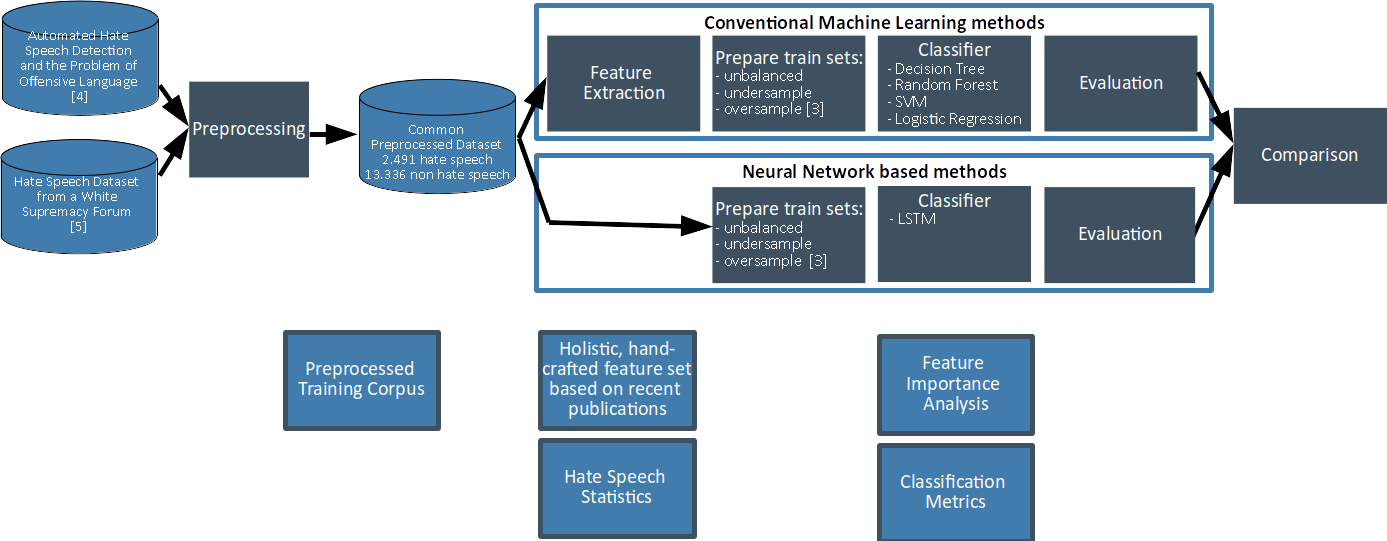
\includegraphics[width=1.0\linewidth]{figures/pipeline.png}
	\caption{Approach}
	\label{fig:overall_pipeline}
\end{figure}

Figure \ref{fig:overall_pipeline} visualizes our approach (on the top) and the resulting novelties achieved through this work (at the bottom). The following chapters describe the different steps in detail. First the data is merged and preprocessed resulting in a preprocessed training corpus. The next step differs between conventional machine learning methods and neural network based approaches. For conventional machine Learning methods an explicit feature extraction is necessary. Therefore achievements of recent publications were combined to build a holistic, hand-crafted feature set. Based on these features, hate speech statictics could be further analyzed. Due to the fact that the common preprocessed corpus is unbalanced, an unbalanced, oversampled and undersampled datasets was created for further investigation. Finally the classifiers are trained, evaluated and the results are compared. Now not only the question whether conventional machine learning methods can outperform neural network based approaches could be answered, but as well which feature were most important for which classifier.

\subsection{Definition of Hate Speech} 
\label{ch:approachA}

Various definitions exist to define hate speech. This work complies with the definitions provided by the two datasets used to label the documents. 

\begin{defStrich}[Ona De Gibert et al.]
	Hate speech is commonly defined as any communication that disparages a target group of people based on some characteristic such as race, color, ethnicity, gender, sexual orientation, nationality, religion, or other characteristic \cite{DeGibert2020}.
\end{defStrich}

\begin{defStrich}[Thomas Davidson et al.]
	A language that is used to expresses hatred towards a targeted group or is intended to be derogatory, to humiliate, or to insult the members of the group \cite{ThomasDavidson2020}.
\end{defStrich}

One can conclude that hate speech is always targeted towards a specific group with the intention to infringe others dignity, often based on group characteristics like race, color or gender. 

\subsection{Data}
\label{ch:approachD}

There are two data sets used for the project. The first one uses data from the \textit{Twitter API} \cite{ThomasDavidson2020}\footnote{https://github.com/t-davidson/hate-speech-and-offensive-language}. It consists of a sample of around 25k tweets that were identified as hate speech based on a previously composed hate speech lexicon without regarding context information. Subsequently, each document in the corpus got labeled with one of the three categories \textit{hate speech}, \textit{offensive language} or \textit{neutral}. Therefore the data set follows a classical ternary clas\-si\-fi\-ca\-tion style. The workers were instructed to follow predefined definitions of each category and to take context information into consideration. Each tweet was assessed and labeled by three or more workers. The majority of tweets were classified as offensive language (76\% at 2/3, 53\% at 3/3), only 5\% were coded as hate speech. The data is provided offline as a CSV or pickle file. 

The second data set uses data from the \textit{White Supremacy Forum} \cite{DeGibert2020}\footnote{https://github.com/Vicomtech/hate-speech-dataset}. One document represents a sentence that is either labeled as hate or not hate. In total, 1.119 sentences containing hate and 8.537 sentences being non-hate are provided. Once again the documents were labeled manually by human actors following previously specified guidelines, on request additional context information was provided. The documents are given offline as normal text files with annotations stored in a separate CSV file. 

\subsection{Preprocessing}
\label{ch:approachB}



\subsection{Features}
\label{ch:approachC}

For the conventional Machine Learning methods we built a hand-crafted feature set. The selection of features is based on recent works \cite{Watanabe2018} and \cite{Fortuna2018}. In the following the feature groups, the extraction process and the evaluation approach for the feature importances are introduced.

\subsubsection*{Feature groups}

Our feature set consists of features from the following five groups:
\begin{itemize}
	\item Unigram features \cite{ThomasDavidson2020, Fortuna2018, Gaydhani2018, Malmasi2017, Oriola2020}
	\begin{itemize}
		\item N-grams
		\item Dictionaries based on TF-IDF
	\end{itemize}
	\item Semantic features \cite{ThomasDavidson2020, Watanabe2018}
	\begin{itemize}
		\item Number of exclamation/question/full stop marks
		\item Number of capitalized words
		\item Number of laughing expressions
	\end{itemize}
	\item Pattern features \cite{Fortuna2018, Oriola2020}
	\begin{itemize}
		\item PoS-tag patterns
	\end{itemize}
	\item Topic classification \cite{Fortuna2018}
	\begin{itemize}
		\item Latent Dirichlet Allocation
	\end{itemize}
	\item Sentiment-based features \cite{Fortuna2018, Oriola2020}
	\begin{itemize}
		\item Polarity scores based on Vader
	\end{itemize}
\end{itemize}

\subsubsection*{Feature extraction}
% Reusable pipeline
The feature extraction of the previously mentioned features is done within a reusable pipeline, which makes it easy to add new features. Each feature is implemented as a class following a predefined structure. By adding the feature class to a list in the Feature\-Extractor the feature is automatically extracted as part of the pipeline. The pipelines input are the data instances as text and the output is a dataframe containing all extracted features as numerical values.

\subsubsection*{Feature importances}
% Feature importances

\subsection{Classifiers}
\label{ch:approachE}

This chapter deals with the classifiers and their integration into the project.

Each classifier is trained on the training set and evaluated on the test set. So the same steps are necessary for each classifier. That is why a reusable pipeline is developed. The pipeline is developed with the Open Closed principle in mind. It is open for extensions and closed for changes. So when adding a new classifier only a few lines of code need to be adapted and steps such as finding the optimal model through hyperparameter tuning and the evaluation are done automatically as part of the pipeline.

As the methods need it, there are slight differences between the training of the classical Machine Learning methods and the neural network based approaches. Figure \ref{fig:classifier_pipeline} illustrates this.

\begin{figure}[ht]
	\centering
	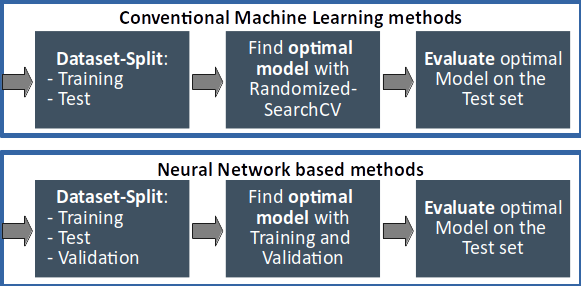
\includegraphics[width=0.7\linewidth]{figures/classifier_pipeline.png}
	\caption{Classifier pipeline}
	\label{fig:classifier_pipeline}
\end{figure}

For the classical Machine Learning methods the dataset is split into training (0.8) and test set (0.2). For finding the optimal model Randomized\-SearchCV is executed on the defined hyperparameter search space. The hyperparameter search space was chosen based on the classifiers doc\-u\-men\-ta\-tion, papers and by an empirical examination. For the decision tree \cite{mantovani2019empirical} and for the random forest \cite{probstHyperparametersTuningStrategies2019} were observed. Finally the model is evaluated on the test set.

TODO: Description for LR, SVM how is the hyperparameter search space set?

For neural network based approaches the dataset is again split into training (0.8) and test set (0.2). Then the training set is further split up into training (0.8) and validation (0.2). In the next step the optimal model is found by using the training and the validation set. The final step is equal to the final step in classical Machine Learning, were the model is evaluated.

To enable a performant execution we use Pythons multiprocessing library to parallelize the execution.

In this work we compare five classifiers on the different datasets (unbalanced, undersampled, oversampled). Four of them are classical Machine Learning methods (Decision Tree, Random Forest, SVM, Logistic Regression) and one neural network based approach (LSTM).


\subsection{Evaluation}
\label{ch:approachF}

For evaluating the classifiers standard metrics such as accuracy, precision, recall and F1 score are used.

The accuracy specifies how many data instances are correctly classified. Only looking at the accuracy, is not that informative, because generally lots of instances are correctly classified as non hate speech, which leads to a high accuracy.

That is why also precision and recall are observed. Precision specifies how many of the predicted hate speech instances are really hate speech. A low precision means that there are lots of instances classified as hate speech, although they are not. So looking at the precision enables to detect if the trained model could built a censoring system and undermine the freedom of speech. The recall specifies how many hate speech instances are correctly classified by the model. A low recall means that there are lots of false negatives (lots of hate speech instances are not detected).

For taking into account precision and recall one can look at the F1 score. 

